\section{Radius Calculation}
To calculate the radius \mathr out of the radian measure \mathl and the angle \mathphi (the difference between the endpoint angle and the starting angle) the
basic equation~\ref{eq:peri} for calculating the perimeter of a circle was settled as starting point. Equation~\ref{eq:radi} shows the final result of the
formula transformations. Figure \ref{fig:arc} shows the parameters of the calculation. For more information see \cite{wikipedia:Kreisbogen}.

\begin{figure}[h]
\centering
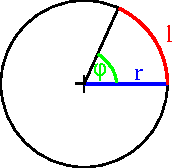
\includegraphics[]{arc}
\caption{Arc showing the parameters of the calculation.}
\label{fig:arc}
\end{figure}

\begin{flalign}
U &= 2\cdot r\cdot \pi && && && U \ldots \text{perimeter}\label{eq:peri}\\
\frac{U}{l} &= \frac{2\cdot r\cdot \pi}{\varphi\cdot r} &&\Rightarrow && U = 2\cdot l\cdot \frac{\pi}{\varphi}  && r \ldots \text{radius}\\
2\cdot l\cdot \frac{\pi}{\varphi} &= 2\cdot r\cdot \pi && && && l \ldots \text{radian measure}\\
r &= \frac{l}{\varphi} && && && \varphi \ldots \text{angle}
\label{eq:radi}
\end{flalign}

To calculate the angle, it is essential to differentiate between left and right curve:
\begin{description}
    \itemsep-2pt
    \item[left:] $\varphi = \varphi_{out} - \varphi_{in}$
    \item[right:] $\varphi = \varphi_{in} -\varphi_{out}$
\end{description}
where \mathphiout is the output angle and \mathphiin the input angle.

\section{End Point Calculation}
The next formula transformations will show how the endpoint coordinates are calculated in all three cases, namely left curve, right curve, and straight
track.

\subsection{Straight Track}

The situation for a straight track is shown in figure \ref{fig:StraightTrack}.
%
\begin{figure}[h]
\centering
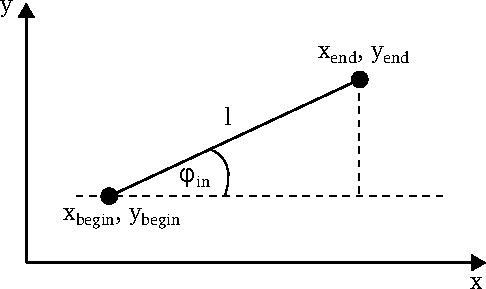
\includegraphics[]{StraightTrack}
\caption{The parameters of a straight track.}
\label{fig:StraightTrack}
\end{figure}
%
For any straight trails equation~\ref{eq:straightx} and equation~\ref{eq:straighty} can be used. Since it is a straight trail, the input angle and the output
angle are the same.

\begin{flalign}
x_{end} &= x_{begin} + l\cdot \cos{(\varphi_{in})} \label{eq:straightx}\\
y_{end} &= y_{begin} + l\cdot \sin{(\varphi_{in})} \label{eq:straighty}
\end{flalign}

\subsection{Curves}

Since every track piece exactly has one radius, it can be seen as an isosceles triangle. The isosceles sides have the length of radius \mathr, whose
calculation is shown in equation~\ref{eq:radi}.To calculate the difference between starting point and endpoint the sine and cosine functions will be used. So
in addition to the length of the track between starting point and endpoint there is a need for the angle of that track.

For the slightly more complicated calculation of the end point of a curve, first of all the coordinates of the center of the circle was calculated (as
sort of reference point). To get a better idea from where this formulas originate, have a look at figure~\ref{fig:curve_left} and
figure~\ref{fig:curve_left_rotated}. Sine and cosine roles are switched due to the fact that the input and output angles are relative to the negative y-axis. So
there is a rotation of $\frac{\pi}{2}$

\begin{flalign}
x_{origin} &= x_{begin} - r\cdot \sin{(\varphi_{in})}\\
y_{origin} &= y_{begin} + r\cdot \cos{(\varphi_{in})}
\end{flalign}

Starting from the origin, the relative distance between center and the endpoint can be calculated. The resulting equations of the endpoint calculation for the
left curve are shown in equation~\ref{eq:leftx} and equation~\ref{eq:lefty}.

\begin{flalign}
x_{end} &= x_{origin} + r\cdot \sin{(\varphi_{out})}\\
y_{end} &= y_{origin} - r\cdot \cos{(\varphi_{out})}\\
x_{end} &= x_{begin} + r\cdot\left(\sin{(\varphi_{out})} - \sin{(\varphi_{in})}\right) \label{eq:leftx}\\
y_{end} &= y_{begin} + r\cdot\left(\cos{(\varphi_{in})} - \cos{(\varphi_{out})}\right)\label{eq:lefty}
\end{flalign}

If we want to calculate the right curve just invert the $+$\ sign in front of $r$. This is shown in equation~\ref{eq:rightx} and equation~\ref{eq:righty}. To
get a better idea of why this difference appears have a look at figure~\ref{fig:curve_right} and figure~\ref{fig:curve_right_rotated}.

\begin{flalign}
x_{end} &= x_{begin} - r\cdot\left(\sin{(\varphi_{out})} - \sin{(\varphi_{in})}\right) \label{eq:rightx}\\
y_{end} &= y_{begin} - r\cdot\left(\cos{(\varphi_{in})} - \cos{(\varphi_{out})}\right)\label{eq:righty}
\end{flalign}

\begin{figure}
\begin{minipage}{0.45\textwidth}
    \centering
    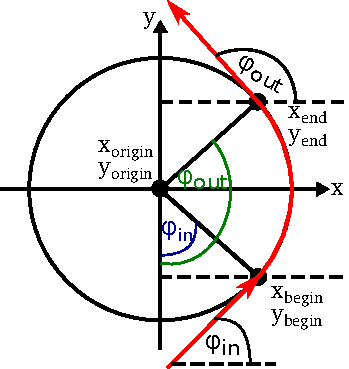
\includegraphics[width=0.6\textwidth]{LeftCurve}
    \caption{Left curve as a track piece.}
    \label{fig:curve_left}
\end{minipage}
\begin{minipage}{0.1\textwidth}
    \centering
    \phantom{}\ \ 
\end{minipage}
\begin{minipage}{0.45\textwidth}
    \centering
    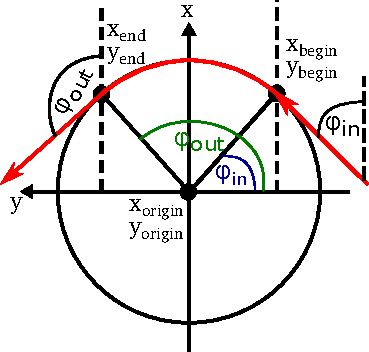
\includegraphics[width=0.6\textwidth]{LeftCurveRotated}
    \caption{Left curve turned around 90\textdegree.}
    \label{fig:curve_left_rotated}
\end{minipage}
\end{figure}

\begin{figure}
\begin{minipage}{0.45\textwidth}
    \centering
    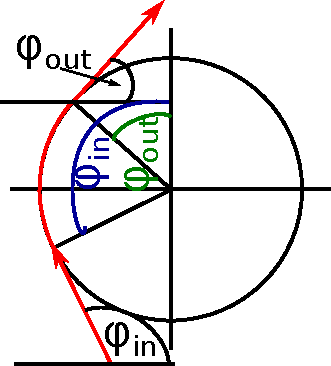
\includegraphics[width=0.6\textwidth]{RightCurve}
    \caption{Right curve as a track piece.}
    \label{fig:curve_right}
\end{minipage}
\begin{minipage}{0.1\textwidth}
    \centering
    \phantom{}\ \ 
\end{minipage}
\begin{minipage}{0.45\textwidth}
    \centering
    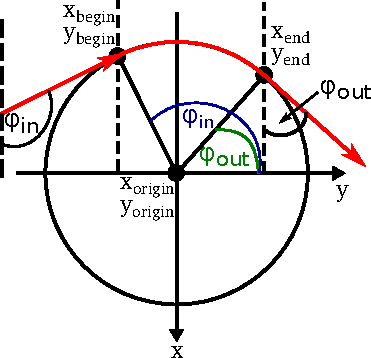
\includegraphics[width=0.6\textwidth]{RightCurveRotated}
    \caption{Right curve turned around -90\textdegree.}
    \label{fig:curve_right_rotated}
\end{minipage}
\end{figure}

\section{Car Flip Simulation}

The car flip simulation requires to calculate the centripetal force \cite{wikipedia:CentripetalForce} and the friction force \cite{wikipedia:Friction}. If the
centripetal force gets greater than the friction force, the car will get thrown out of the track. For more information, take a look on the theory about
(un)banked turns, e.g. \cite{UnbankedTurn} and \cite{wikipedia:BankedTurn}. Since the AI is going to receive values from the gyro sensor, we need to transfer
the calculated force to the corresponding sensor values. This will be one of the inputs for the AI.

\begin{flalign}
F_R &= m\cdot g\cdot \mu && F_R \ldots \text{friction force}
\end{flalign}

For calculating the friction force, we have some constant values. The mass $m$ of the car, the gravitational acceleration $g$, and $\mu$ which describes the
friction coefficient. The friction coefficient $\mu$\ could take on different values on different places of the track, but this consideration is a possible
extension for future use. For easier calculation, it will be determined as constant.

An additional problem appears if the wheels are spinning through. In this case, the friction coefficient will change (it gets more tiny). There are cases in
which just one wheel spins through, or two wheels. In these cases the friction force has to be calculated a little bit more complicated. Since only 2 of the 4
wheels of the Carrera car really touch the ground, the total friction force can be calculated as shown in equation \ref{eq:total_friction}. The masses $m_{i}$
can simplified be assumed as $\frac{m}{2}$.

\begin{flalign}
F_{Rs} &= g\cdot \sum\limits_{i=1}^2 \left( m_i\cdot {\mu}_i\right) && F_{Rs} \ldots \text{friction force spin through}  \label{eq:total_friction}
\end{flalign}


 The coefficient can take
on 2 different values:
\begin{enumerate}
    \itemsep0pt
    \item spin through value
    \item normal spin value
\end{enumerate}

The maximum velocity $v_{max}$ with which the car can drive an unbanked curve is shown in equation \ref{eq:max_velocity}. The parameter $r$\ describes the
radius of the curve which was calculated in equation~\ref{eq:radi}. For more information about this equation, take a look at \cite{Kurvenfahrten}.
\begin{flalign}
v &\leq \sqrt{\mu_{Haft} \cdot r \cdot g} \\
v_{max} &= \sqrt{\mu_{Haft} \cdot r \cdot g} \label{eq:max_velocity}\\
\omega_{max} &= \frac{v_{max}}{r} = \frac{\sqrt{\mu_{Haft} \cdot r \cdot g}}{r} = \sqrt{\frac{\mu_{Haft} \cdot g}{r}} \\
\end{flalign}

The actual velocity $v$ of the car is determined by the rotational speed $n$ of the wheels with diameter $d_{w}$, as shown in equation \ref{eq:actual_velocity}.
\begin{flalign}
v &= \omega \cdot r_{w} = 2 \pi n \cdot r_{w} = d_{w} \cdot \pi \cdot n \label{eq:actual_velocity}
\end{flalign}


\section{Gyro Sensor}

The gyro sensor provides 3 values, which represent a rotation in each of the 3 dimensions we know. The mathematical dependencies between $\omega$\ and the
gyro rotation around the z -- axis is defined as follows.

\begin{flalign}
Z_{gyro} = a\cdot \omega && Z_{gyro} \ldots \text{gyro rotation around z-axis}
\end{flalign}

The parameter $a$\ represents a constant factor which is the difference between $\omega$\ and $Z_{gyro}$. In fig.~\ref{fig:forces} you can see which force
shows in which direction. In addition there is an axis of abscissas so you know where the z-axis shows to (for $Z_{gyro}$).

\begin{figure}[h]
    \centering
    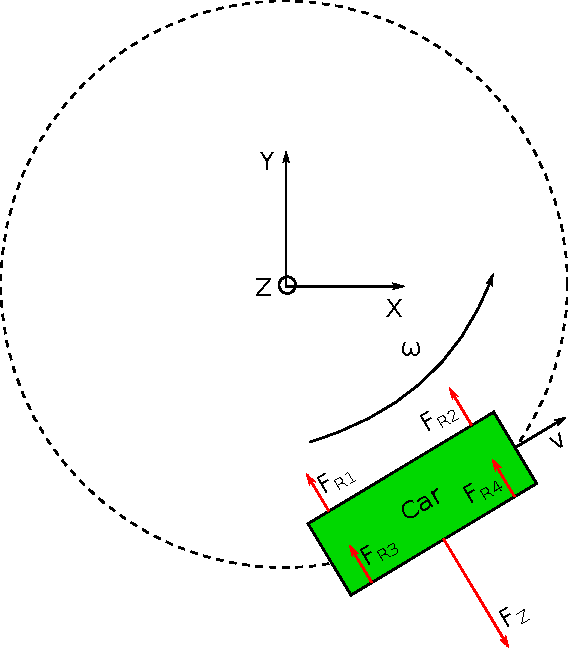
\includegraphics[width=0.34\textwidth]{forces}
    \caption{Forces in a curve.}
    \label{fig:forces}
\end{figure}
